\documentclass[aspectratio=169]{beamer}

\usepackage{tabularx}
\usepackage{booktabs}
\usepackage{colortbl}
\usepackage{media9}
\usepackage{multimedia}
\usepackage{hyperref}
\usepackage{subfigure}
% \usepackage[brazil]{babel}
\usepackage{amssymb}
\usepackage{amsthm,amsfonts}
\usepackage[utf8]{inputenc}
\usepackage{latexsym}
\usepackage{float}
\usepackage[T1]{fontenc}
\usepackage{beamerthemeshadow}
\usepackage{helvet}
\usepackage{graphicx}       % I don't think color.sty is needed.
\usepackage{epstopdf}
\usepackage{listings}
\usepackage{tikz}
\usetikzlibrary{arrows,shapes}
\usepackage{algpseudocode}
\usepackage{algorithm}
\usepackage{algorithmicx}
\usepackage{subfigure}
% \usepackage[brazil]{babel}
\usepackage{amssymb}
\usepackage{amsthm,amsfonts}
\usepackage[utf8]{inputenc}
\usepackage{latexsym}
\usepackage{float}
\usepackage{beamerthemeshadow}
\usepackage{lipsum}
\usepackage{listings}
\usepackage{color}
\usepackage{xcolor}
\usepackage{tikz}
\usetikzlibrary{arrows,shapes}
\usepackage{color, colortbl}
\usepackage{float} 
\floatplacement{figure}{hb} 
\floatplacement{table}{hb} 
\usepackage{placeins} 
\definecolor{Gray}{gray}{0.9}
\usepackage{stfloats}
\usepackage{tabularx}
\usepackage{fancyhdr}

\addmediapath{.}

%  \usetheme{Copenhagen}
\usetheme{Darmstadt}
%    \usetheme{default}
% \usetheme{Antibes}

% \usecolortheme{crane}
\usecolortheme{default}
% \usecolortheme{dolphin}
% \usecolortheme{seagull}
% \usecolortheme{seahorse}

\newcommand{\mc}[2]{\multicolumn{#1}{c}{#2}}
\definecolor{Gray}{gray}{0.85}
\definecolor{LightCyan}{rgb}{0.7,1,1}\setbeamersize{text margin left=10pt,text margin right=10pt}

\newcolumntype{a}{>{\columncolor{Gray}}c}\setbeamertemplate{footline}[frame number]
\newcolumntype{b}{>{\columncolor{white}}c}
\beamertemplatetransparentcovereddynamic

\AtBeginSection[]
{
   \begin{frame}
   \frametitle{Outline}
       \tableofcontents[currentsection]
   \end{frame}
}

\setbeamercolor{block body}{bg=blue!22,fg=black}

\begin{document}

\title[]{\textbf{MODELO ADAPTATIVO PARA PREVISÃO DE DEMANDA POR RECURSOS DE REDE EM PROVEDORES DE INTERNET MODERNOS}}  

\author[Dyego Oliveira]{Dyego Henrique Leonel Oliveira}

\institute{Universidade Estadual do Ceará (UECE)}

\date{Julho 2020} 

\begin{frame}
\titlepage

\end{frame}

% \setcounter{tocdepth}{1}

\begin{frame}
\frametitle{Outline }
\tableofcontents
\end{frame} 

%%%%%%%%%%%%%%%%%%%%%%%%%%%%%%%%%%%%%%
%-------------------------------------
%%%%%%%%%%%%%%%%%%%%%%%%%%%%%%%%%%%%%%

\section{Introdução}

%%%%%%%%%%%%

\subsection{}
\begin{frame}
\frametitle{Introdução}
% \small
\begin{block}{Contexto}
    \begin{itemize}
        \item A Internet tem se tornado uma ferramenta crucial em nossas vidas, pelos serviços modernos de comptuação que operam sobre.
        \item A maioria desses serviços são baseados em:
        \begin{itemize}
            \item Service Level Agreement -- SLA
            \item Internet Access Service -- IAS
        \end{itemize}
        \item Operando através o Internet Service Provider (ISP)
    \end{itemize}
\end{block}


\end{frame}
%%%%%%%%%%%%
\subsection{}
\begin{frame}{Introdução}
    \begin{block}{Desafios}
\begin{itemize}
    \item Todos os tipos de redes buscam por características tais como:
    \begin{itemize}
        \item baixo atraso;
        \item flexibilidade;
        \item resiliência;
    \end{itemize}
    \item Pontos necessários para evoluir o gerenciamento de recursos, flexibilidade, bandwidth e poder personalizar o comportamento de infraestruturas das redes.
\end{itemize}
\end{block}
\end{frame}
%%%%%%%%%%%%

\subsection{}
\begin{frame}
\frametitle{Introdução}
% \small
\begin{block}{MISPs e Demanda Elastica}
    \begin{itemize}
    \item ISPs tendem a evoluir para MISPs (Modern Internet Service Providers), abordando situações como demanda elástica por recursos de rede. 
    \item Os MISPs precisam expandir ou reduzir dinamicamente a alocação de largura de banda (comportamento elástico), permitindo um IAS adequado sob demanda. Evitando problemas de lentidão, interrupção e desconecções. 
    \item Uma abordagem promissora para os MISPs são o desenvolvimento de fatias de redes (slices). Cada fatia pode ter a configuração adequada para melhor atender as necessidades do cliente.
    \item Uma abordagem promisora para lidar com (slices) é o uso de Previsão de Tráfego de Rede.
    \end{itemize}
\end{block}
\end{frame}

%%%%%%%%%%%%

\subsection{}
\begin{frame}
\frametitle{Introdução}
% \small
\begin{block}{Traffic prediction model}
    \begin{itemize}
        \item The analysis of the history of use of network resources allows the understanding of the network's behavior.
        \item This knowledge allows the application of proactive tasks to avoid the problems mentioned above and to plan the network infrastructure.
        \item Traditional traffic prediction models lack adaptability to keep up with changes in the behavior of observations.
        \item MISPs need a model that performs adaptive forecasting to deal with the elastic demand arising from clients behavior.
    \end{itemize}
\end{block}
\end{frame}

%%%%%%%%%%%%

\subsection{}
\begin{frame}
\frametitle{Introduction}
% \small
\begin{block}{Proposal: ANP}
    \begin{itemize}
        \item Adaptive Network Prediction (ANP).
        \begin{itemize}\setbeamertemplate{itemize items}[triangle]\small
        	\item The ANP model allows for an adequate allocation of network resources and strategic planning of its infrastructure.
            \item Goals:
            \begin{itemize}\setbeamertemplate{itemize items}[square]\small
            	\item Adapt the utilization of distinct means of bandwidth for cycles intervals.
            	\item Perform a sequence of adjustments to reach suitable values of generalization.
            \end{itemize}
        \end{itemize}
        \item Through ARIMA and NNAR, the ANP makes adjustments in seasonality, trend and removes error cycles in the time series.
        \item Experiments and results:
        \begin{itemize}\setbeamertemplate{itemize items}[triangle]\small
        	\item The experiments were carried out using a six-month real bandwidth demand data set from the Universidade Estadual do Ceará (UECE - Brazil).
        	\item Minimizes the error rate of the predicted values, reaching 30\% improvement when compared to the existing network forecast models.
        \end{itemize}
    \end{itemize}
\end{block}
\end{frame}

%%%%%%%%%%%%%%%%%%%%%%%%%%%%%%%%%%%%%%
%-------------------------------------
%%%%%%%%%%%%%%%%%%%%%%%%%%%%%%%%%%%%%%
\section{Fundamentação Teórica}
\subsection{}

\begin{frame}{Série Temporal}
    \begin{itemize}
        \item 
    \end{itemize}
\end{frame}

\begin{frame}{Frame Title}
    
\end{frame}

%%%%%%%%%%%%%%%%%%%%%%%%%%%%%%%%%%%%%%
%-------------------------------------
%%%%%%%%%%%%%%%%%%%%%%%%%%%%%%%%%%%%%%

\section{Related Work}

\subsection{}
\begin{frame}

\frametitle{Related Work}

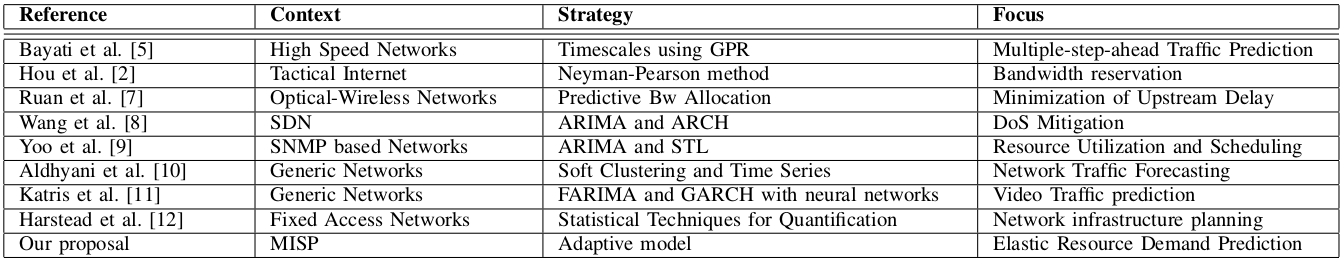
\includegraphics[width=0.99\textwidth,angle=0]{tableRelatedWork.png}

\begin{itemize}\footnotesize
    \item No paper in the literature focused on the design of an adaptive bandwidth prediction model for elastic demand in MISPs.
    \item To improve the prediction process, our proposal performs several tasks that create a standardized sample model that evolves the prediction process of existing techniques, reducing the computational time to create the models, as well as their accuracy.
\end{itemize}

\end{frame}

%%%%%%%%%%%%%%%%%%%%%%%%%%%%%%%%%%%%%%
%-------------------------------------
%%%%%%%%%%%%%%%%%%%%%%%%%%%%%%%%%%%%%%

\section{Proposal}

%%%%%%%%%%%%

\subsection{}
\begin{frame}
\frametitle{ANP Model}
\begin{block}{Behavior}
    \begin{itemize}\small
    \item The ANP model aims to adjust the data referring to the use of bandwidth to the elastic demand scenarios, allowing a better performance of the existing prediction techniques.
    %\item Essas técnicas lidam com questões de sazonalidade e tendência, mas geralmente não atingem fatores de correção adequados, deixando de prever o comportamento dos dados adequadamente, especialmente em situações de demanda elástica.
    %\item These techniques deal with seasonality and trend issues, but usually they do not attain suitable correction factors, failing to predict the data behavior properly, specially in elastic demand situations.
    \item The ANP model performs the following tasks sequentially:
    \begin{itemize}\setbeamertemplate{itemize items}[triangle]
        \item Data decomposition.
        \item Stationarity test. 
        \item Cycles removal.
    \end{itemize}
    \item After being preprocessed by the ANP model, data may be processed a chosen prediction technique. The following figure illustrates the ANP execution process.
    \end{itemize}
\end{block}

\centering
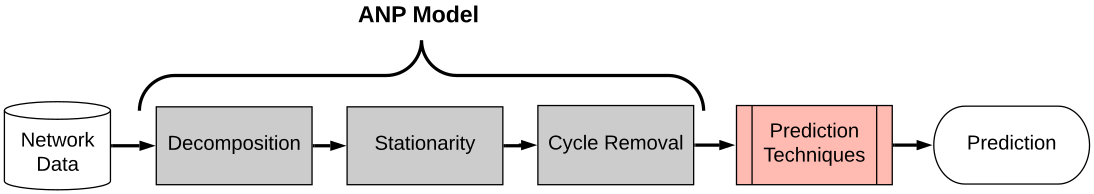
\includegraphics[width=0.8\textwidth,angle=0]{ANPModel.png}

\end{frame}

%%%%%%%%%%%%

%%%%%%%%%%%%%%%%%%%%%%%%%%%%%%%%%%%%%%
%-------------------------------------
%%%%%%%%%%%%%%%%%%%%%%%%%%%%%%%%%%%%%%

%%%%%%%%%%%%

\section{Results}

%%%%%%%%%%%%

\subsection{}
\begin{frame}
\frametitle{Results}
\small
\begin{block}{Workload}
\begin{itemize} \small
    \item The dataset used described the bandwidth usage of the central backbone of the UECE.
    \item The data was collected through real time network monitoring every 60 minutes, during six months. A period of 24 hours defines a cycle, so, all the dataset is composed by 4320 cycles.
\end{itemize}
\end{block}

\begin{block}{Training and test samples}
\begin{itemize} \small
    \item The technique Time Series Cross-Validation (TSCV) was applied due to the dependency of the time series.
    \item The TSCV was used to model the samples in order to input them for prediction.
    \item The HoldOut method was used to select the subsets of Training and Test.
    \item We applied first 72 samples as training set, second 144 samples for the training and so on (72, 144, 216, . . . ).
\end{itemize}
\end{block}
\end{frame}

%%%%%%%%%%%%

\subsection{}
\begin{frame}
\frametitle{Results}
\small
\begin{block}{Comparison}
\begin{itemize} \small
    \item The ANP model is used as previous step to the application of the prediction technique.
    \item To measure the benefits of the ANP in the modeling and predition capacity of the ARIMA and NNAR techniques, we compare their performance with and without the application of the ANP model. 
\end{itemize}
\end{block}

\begin{block}{Metric}
\begin{itemize} \small
    \item The metric used to evaluate the performance of the proposal in a period T is the Root Mean Squared Error (RMSE), follows the equation below, where ŷ t is the predicted value and y t is the real values of bandwidth usage in time t.
\end{itemize}

\begin{equation}
RMSE(T) = \frac{1}{\sqrt{T}} (\sum_{t=1}^{T} (\hat{y}_t - y_t)^2)^\frac{1}{2}    
\end{equation}

\end{block}
\end{frame}

%%%%%%%%%%%%

\subsection{}
\begin{frame}
\frametitle{The ANP model improves the performance of prediction techniques}
\small

\begin{itemize}\footnotesize
 \item ARIMA and NNAR reach high values of RSME in several moments, representing the impact of the elastic demand situation in the prediction capacity of both techniques.
 \item When ARIMA and NNAR techniques are applied together with the proposed ANP model, the performance of both techniques increase (lower prediction errors), reaching similar values.
\end{itemize}

\vspace{-0.2cm}

\centering
\begin{figure}[!htb]
\centering
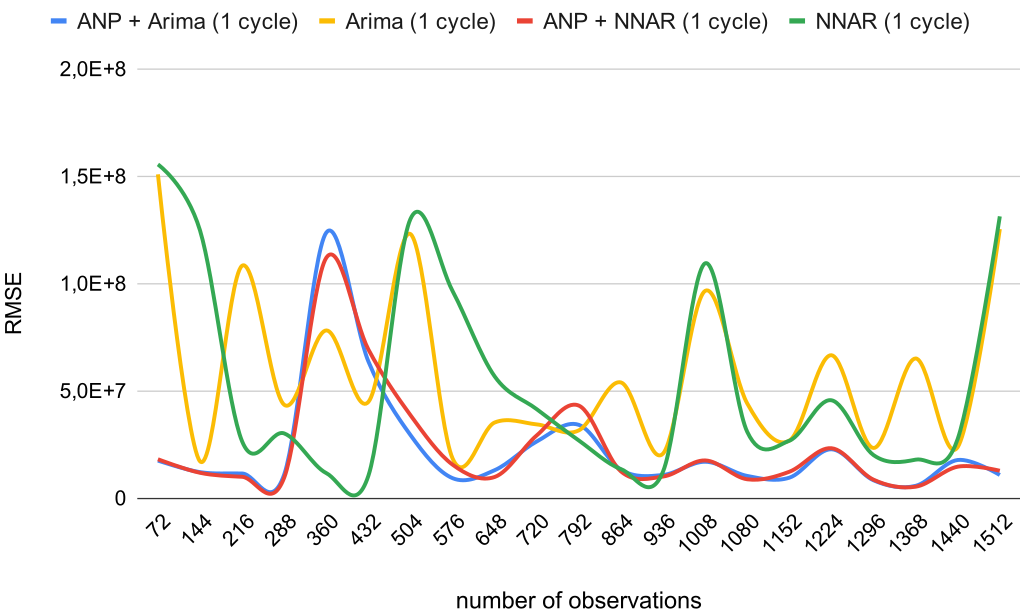
\includegraphics[height=0.35\textwidth,angle=0]{figura6.png}
\end{figure}

\end{frame}

%%%%%%%%%%%%

\subsection{}
\begin{frame}
\frametitle{The ANP model favors adaptability to behavioral changes}
\small

\begin{columns}[T] % align columns
\begin{column}{.4\textwidth}
\begin{itemize}\footnotesize
    \item The ANP model can accompany the samples of the time series of the dataset, following the seasonality and amplitude fluctuations, giving the importance of the samples variation (with approximately 2, 4, 6 and 8 weeks)
    \item Moreover, the ANP model reduced the computational processing for the training phase in around 85\% using ARIMA and 12\% applying NNAR. This fact indicates that the ANP model is capable to reduce the processing time for the prediction techniques, enabling its application in real time prediction scenarios.
\end{itemize}
\end{column}%

\hfill%

\begin{column}{.6\textwidth}
\centering
\begin{figure}[!htb]
\centering
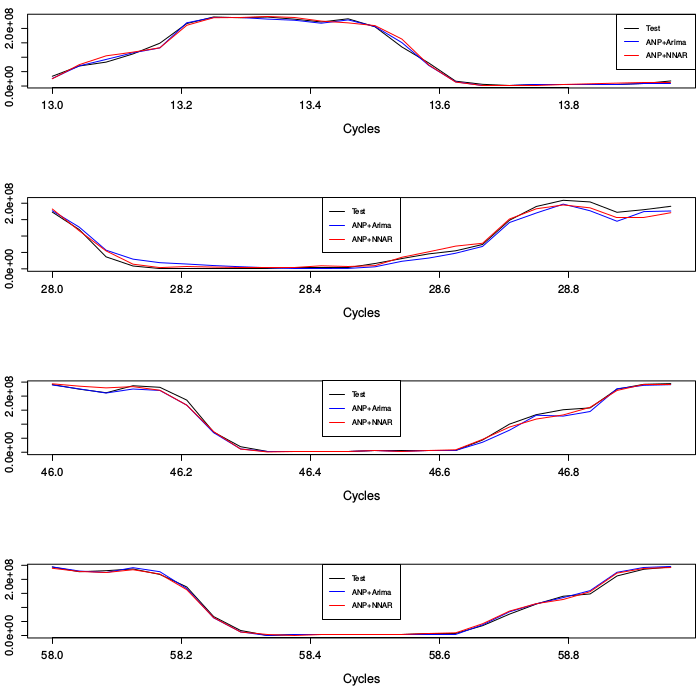
\includegraphics[height=0.7\textwidth,angle=0]{figura7.png}
\end{figure}
\end{column}%
\end{columns}

\end{frame}

%%%%%%%%%%%%

%%%%%%%%%%%%%%%%%%%%%%%%%%%%%%%%%%%%%%
%-------------------------------------
%%%%%%%%%%%%%%%%%%%%%%%%%%%%%%%%%%%%%%

%%%%%%%%%%%%

\section{Conclusion}

%%%%%%%%%%%%

\subsection{}
\begin{frame}
\frametitle{Conclusion e Future Work}
\small
\begin{block}{Conclusion}
\begin{itemize} \small
\item The ISPs tend to evolve to MISPs, in order to deal with situations that can affect the QoS of service delivery.
\item Problem: improve the existing prediction techniques, turning them in a efficient approach to overcome situations of elastic demand of network resources.
\item The proposed model, called ANP, is used as previous step to the application of the prediction technique.
\item The experiments performed show that the model ANP together with a prediction technique evolved the prediction capacity, reducing around 30\% the RMSE error rate.
\end{itemize}
\end{block}

\begin{block}{Future Work}
\begin{itemize} \small
\item Extend the prediction approach, including issues related to independent variables, which can generate a higher capacity of knowledge about the elastic demand behavior.
\end{itemize}
\end{block}

\end{frame}

%%%%%%%%%%%%


\subsection{}
\begin{frame}
\frametitle{Thank you !}
% \small

\begin{block}{Acknowledgment}\small
The authors would like to thank FUNCAP, CAPES and
CNPq for their financial support.


%This work was partially supported by CNPq (grants n. 307118/2017-7 and 405642/2016-4). This work is part of the INCT of the Future Internet for Smart Cities (CNPq 465446/2014-0, Coordena\c{c}\~{a}o de Aperfei\c{c}oamento de Pessoal de N\'{i}vel Superior - Brasil (CAPES) - Finance Code 001, and FAPESP 2014/50937-1 and 2015/24485-9).

\end{block}

\begin{block}{Contact}\small
Email: \{dyego,mardoniovf,thelmo,celestino,rafaellgom\}@larces.uece.br
\end{block}

\end{frame}
%%teste
%%%%%%%%%%%%

\end{document}